
\subsection{Amdahl}
\label{sec:amdahl}

Amdahl's law is used to estimate the the total speed up gained from speeding up a single segment. $s_v$ is the speed up in the chosen segment or component. Here: the moving window integration filter. It takes up the fraction $r$ of the total computation time. The total speed up $s_t$ gained by speeding up one segment by a factor $s_v$ is given by Amdahl's law:

\begin{equation}
    s_t = \frac{s_v}{1+(s_v-1) r}
\end{equation}

\textbf{r-value:} In assignment 1, we found that the filters took up 66.2 \% of the total computation time. The moving window integration filter is major culprit. Assuming that this filter accounts for 75 \% of the filter time, we estimate $r = 0.75 \times 0.662 = 0.4965 \approx$ 0.5. Hence this single filter accounted for half the total computation time.\\

With the calculated $r$, we can plot the possible gain from speeding up the moving window integration filter, seen in figure \ref{fig:amdahl}.\\

\textbf{Upper bound:} Examining Amdahl's Law, we see that when $s_v$ gets sufficiently large (and for $r \ne 0$), it can be simplified to $\frac{s_v}{s_vr}$:

\begin{equation}
    s_t = \frac{s_v}{1+(s_v-1) r} \rightarrow \frac{s_v}{s_v r} \text{ for } s_v \gg 1
\end{equation}

\textbf{Best case:} For $r = 0.5$, $s_t$ asymptotically approaches $\frac{2s_v}{s_v} = 2$. This asymptote can be seen in figure \ref{fig:amdahl}. Hence no matter how large the speedup $s_v$, it can at best halve the total computation time. \\

\textbf{Our case:} Applying Amdahl's law for $r=0.5$ and $s_v = 25$, we compute the total speed up $s_t = 1.92$. This is close to the maximum speed up, and therefore acceptable. The data point $(s_v, s_t) = (25, 1.92)$ is seen in figure \ref{fig:amdahl}.

\begin{figure}[H]
    \centering
    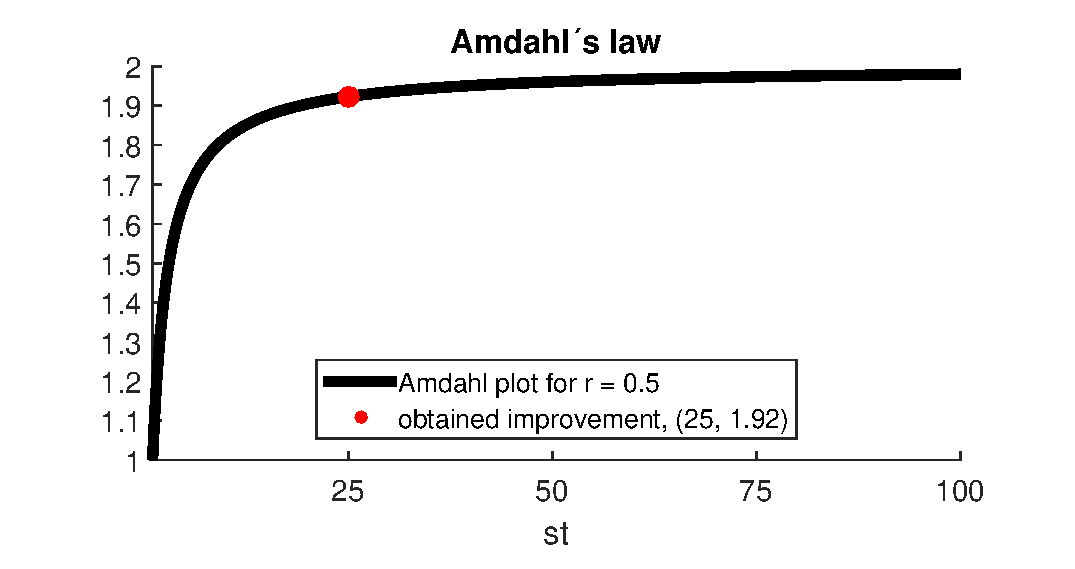
\includegraphics[width=0.8\textwidth]{3Results/fig/Amdahl.eps}
    \caption{Total speed up $s_t$ for the ECG program by speeding up the moving window integration filter by a factor $s_v$.}
    \label{fig:amdahl}
\end{figure}
